\documentclass{article} % For LaTeX2e
\usepackage{nips_adapted,times}
\usepackage{hyperref}
\usepackage{url}
\usepackage{graphicx}
\usepackage{booktabs}
\usepackage[font=small,labelfont=bf]{caption} % Required for specifying captions to tables and figures
\usepackage{float}
\usepackage[square,numbers]{natbib}
\usepackage{amsmath}
\bibliographystyle{abbrvnat}

\title{Experiments with Knowledge Distillation for building lightweight Deep Learning Models}


\author{
	Vaibhav Thakkar \\
	170778 \\
	\href{vaithak@iitk.ac.in}{vaithak@iitk.ac.in}\\
	\And
	Arpit Kumar Jhunjhunwala \\
	170149 \\
	\href{mailto:arpitjjw@iitk.ac.in}{arpitjjw@iitk.ac.in} 
}

% The \author macro works with any number of authors. There are two commands
% used to separate the names and addresses of multiple authors: \And and \AND.
%
% Using \And between authors leaves it to \LaTeX{} to determine where to break
% the lines. Using \AND forces a linebreak at that point. So, if \LaTeX{}
% puts 3 of 4 authors names on the first line, and the last on the second
% line, try using \AND instead of \And before the third author name.

%(1) Problem description/motivation
%(2) Literature review and description of prior work on the problem
%(3) Novelty of your work as compared to prior work (only for projects for which this applies)
%(3) Description of tools/softwares you used
%(4) Experimental results including description of data you have used (if any)
%(5) Things that you learned while doing the project.
%(6) Possible future work


\newcommand{\fix}{\marginpar{FIX}}
\newcommand{\new}{\marginpar{NEW}}

\nipsfinalcopy

\begin{document}
	
	
	\maketitle
	\begin{center}
		\textbf{Disclaimer}\\
		The work carried out in this project has not been re-used from any another course project at IITK or elsewhere, or any other project done elsewhere (e.g., an internship).\\
		Further we have acknowledged all the sources used and cited them in the reference section.
		
	\end{center}
	\section{Introduction and Motivation}
	Deep Learning has been successful in a variety of areas and applications, some of the classic ones being Robots, Chatbots and Face Recognition; some examples of surprising applications being Google's DeepMind AlphaFold2 for Protein Folding \cite{alphafold},  Lip Reading, Agriculture \cite{Kamilaris_2018} and many more. The great success of deep learning is mainly due to its capability to encode large-scale data and to maneuver billions of model parameters. However, it is a challenge to deploy these cumbersome deep models on devices with limited resources, e.g., mobile phones and embedded devices, not only because of the high computational complexity but also the large storage requirements. 
	
	The main aim of knowledge distillation is to give the power to deploy lightweight models on such devices without sacrificing much on accuracy and performance. Student models taught using this technique performed better than the student models trained using only the training data. 
	
	We will explore more insights into this technique in general using empirical analysis on several datasets and models combination.
	\section{Problem Description}
	A standard classification model is trained using the hard labelelled data, whereas a student model trained using knowledge distillation follows the given procedure as proposed by Hinton et. al \cite{hinton2015distilling}:
	
	During training along with the labels of data, the student also uses the probabilities outputted by the teacher model, the benefit of using these probabilities is that it contains more information than just hard labels, as it also tells the similarity and differences between classes (this is called as the dark knowledge).
	\newpage
	
	\begin{center}
		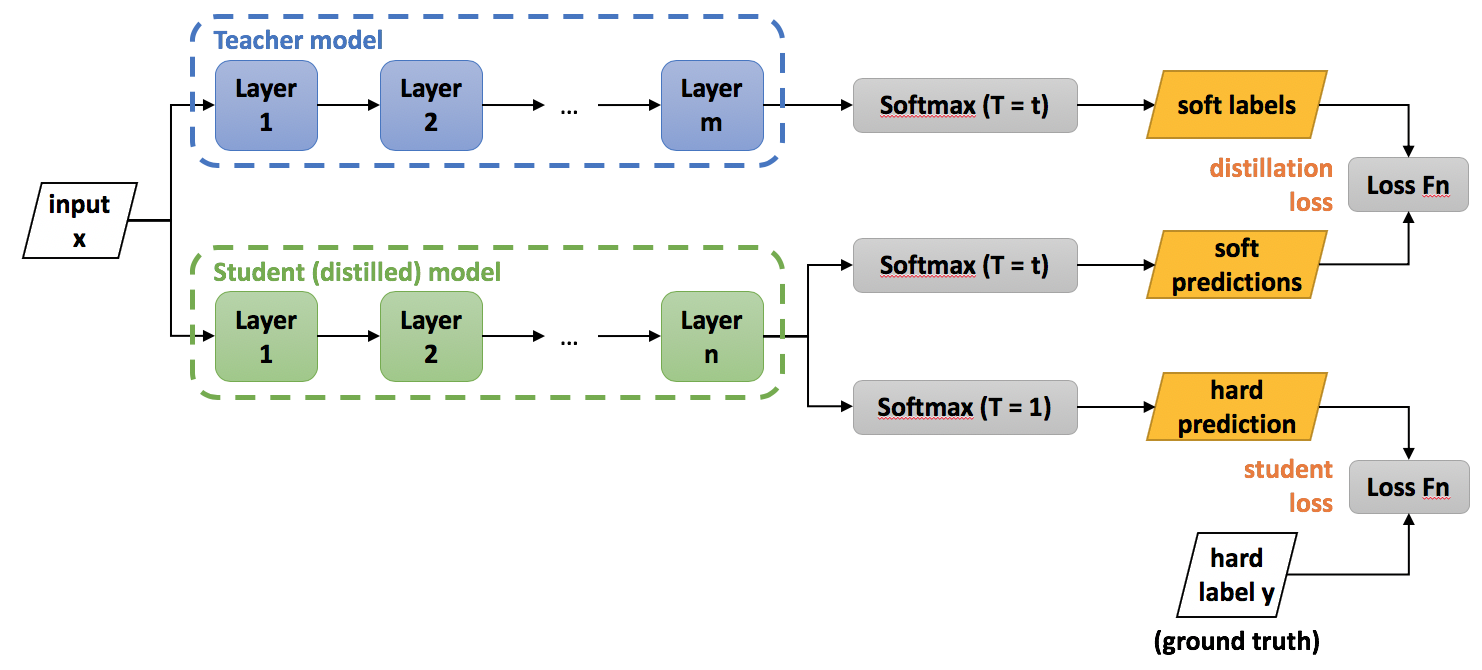
\includegraphics[width=\linewidth]{fig/kd_12}
		\captionof{figure}{Overview of logit based     knowledge distillation. Source: \textbf{\href{https://medium.com/neuralmachine/knowledge-distillation-dc241d7c2322}{medium.com}}}
	\end{center}
	
	For transferring the dark knowledge from teacher to student, the logits from the pre-softmax layer is used to output the soft probabilities at a temperature T ($\geq 1$), using the following equation:
	\begin{equation}
		\operatorname{softmax}\left( \frac{a}{T} \right) = \Big[ \frac{\exp(a_i / T)}{\sum_{j} \exp(a_j / T)} \Big]_i
	\end{equation}
	
	An example of why soft predictions at raised temperature are useful:
	\begin{center}
		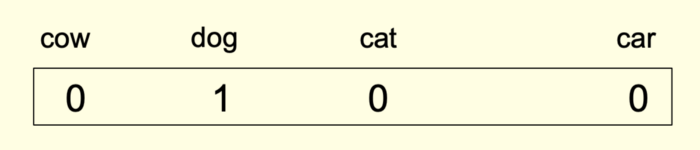
\includegraphics[width=0.48\linewidth]{fig/kd_7}
		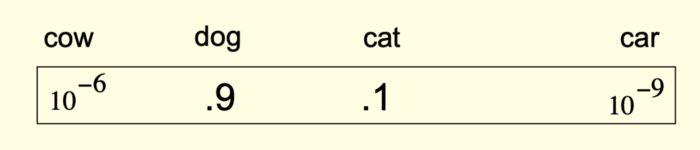
\includegraphics[width=0.48\linewidth]{fig/kd_8}
		\captionof{figure}{a) Hard Labels  b) Soft Predictions at T = 1}
	\end{center}
	\begin{center}
		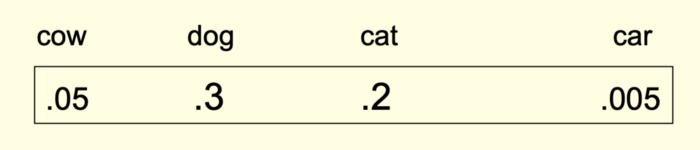
\includegraphics[width = 0.5 \linewidth]{fig/kd_9}
		\captionof{figure}{Soft Prediction at raised temperature T}
	\end{center}
	
	Therefore the final loss function is: 
	\begin{equation}\label{eq:kd}
		\mathcal{L}_{student} = (1 - \alpha)\mathcal{L}_{sl} + \alpha\mathcal{L}_{KD} 
	\end{equation}
	
	Where $a_s, a_t$ are logits from layer of student and teacher model respectively, and: 
	\begin{equation} 
		\begin{aligned}
			\mathcal{L}_{sl} &= \mathcal{H}\left(\operatorname{softmax}\left(a_{s}\right), y\right) \\
			\mathcal{L}_{KD} &= T^{2} \cdot K L\left(y_{s}, y_{t}\right) \\
			y_{s} &= \operatorname{softmax}\left(\frac{a_{s}}{T}\right) \\
			y_{t} &= \operatorname{softmax}\left(\frac{a_{t}}{T}\right) 
		\end{aligned}
	\end{equation}
	So, in a way the student is also trying to mimic the output of the teacher.
	
	\section{Literature review}
	\begin{itemize}
		\item The idea of Knowledge distillation was first proposed by Caruana et al. \cite{10.1145/1150402.1150464} in 2006 for the purpose of model compression. In 2015, one of the most influential KD paper was published by Hinton et al. \cite{hinton2015distilling} which inspired many other variants. The class probabilities produced by the more complex Teacher model are used as ‘soft targets’ in addition to the available class labels to train the Student model. 
		Our problem formulation in the above section is mainly referenced from this paper.
		
		\item A lot of recent works use the knowledge from intermediate layers of the teacher to improve the performance of the student model. 
		In the Fitnets \cite{fitnets} architecture, the student model is thinner but deeper than the teacher. The paper proposes a 'Hint-based training' method in which a layer ('guided') of the student learns the output of an intermediate layer ('hint') of the teacher using a fully-connected or convolutional regressor in a 2-stage training process. In this method the student's guided layer tries to directly learn the activations of the hint layer using the MSE loss. 
		
		\item Some recent works have proposed indirect ways of learning the intermediate feature maps. These methods perform distillation on derived maps. Zagoruyko and Komodakis \cite{attention} proposed the use of pair of attention maps derived from the intermediate layers of the student and teacher models. These pair of maps are computed across several layers and a transfer loss is minimized in addition to the standard cross-entropy loss. 
		Yim et al. \cite{yim2017gift} proposed the use of Flow of Solution Procedure (FSP) matrix calculated from the feature maps to transfer knowledge between the intermediate layers. 
		
		\item While most of the KD methods uses a Teacher model, Yuan et al. \cite{teacherfree} proposed a Teacher-free framework which uses a pre-trained student model as the Teacher. A second proposed method uses a manually designed virtual teacher with 100\% accurate soft predictions on training data.
		Yuan et al. provided a theoretical justification as to why these two methods work by examining KD from the perspective of Label Smoothing Regularization (LSR).\\
		The overall loss function when applying LSR to the student model is given by:\\
		\begin{equation}\label{eq:lsr}
			\mathcal{L}_{Student}=(1-\alpha)\mathcal{H}_{Student}+\alpha\mathcal{L}_{KL}(u,p_{student})
		\end{equation}
		where $\mathcal{H}_{Student}$ is the standard cross entropy loss of the student and $\mathcal{L}_{KL}(u,p)$ is the KL divergence loss between a uniform distribution $u$ and the predicted class probability distribution $p$.\\
		Eq.\eqref{eq:kd} and Eq.\eqref{eq:lsr} have similar form which which suggests that Knowledge-Distillation is a learned Label Smoothing Regularization.
		
		\item 
		Mirzadeh et al \cite{assistant} introduced the usage of Teacher assistants (TA) for bridging the complexity gap between student and teacher model. The idea was that the Teacher model first teaches the TA model, and then the TA model teaches the student model.
		
		\item Knowledge Distillation can also be used to build compact and efficient object detection networks. One such framework was proposed by Guobin Chen et al. \cite{chen2017learning} in 2017. 
		
	\end{itemize}
	% The probability $p(i)$ of class $i$ is calculated from the logits $z_{i}$ as:
	% \begin{center}
	% $p^{T}(i)=\frac{exp(z_{i}/T)}{\sum_{j}exp(z_{j}/T)}$
	% \end{center}
	
	% where $T$ is the temperature used to smooth the probability distribution of classes. When $T$ = 1, we get the standard softmax function. \\
	% The weighted loss function, incorporating both student and distillation losses is given by:\\
	% \begin{equation}\label{eq:kd}
	% \mathcal{L}_{student}=(1-\alpha)\mathcal{H}_{student}+\alpha\mathcal{L}_{KL}(p^{T}_{student},p^{T}_{teacher})
	% \end{equation}
	% where $\alpha$ is the weight hyperparameter, $\mathcal{H}_{Student}$ is the standard cross entropy loss of the student and $\mathcal{L}_{KL}$ is the Kullback-Leibler divergence (KL divergence) loss between the smooth (controlled by T) probability distribution over the classes of the teacher and student models. \\ 
	% By including the distillation loss, we provide student, knowledge about the similarity between the classes which the teacher has to learn from scratch. This 'dark knowledge' is transferred to student in the distillation process.
	
	
	
	\section{Our Experiments}
	\subsection{Datasets}
	\begin{itemize}
		\item \textbf{MNIST Dataset of Handwritten Digits}: \cite{lecun2010mnist} This dataset consists of a training set of 60,000 examples, and a test set of 10,000 examples. All the images are in grayscale and are of size 28x28 with a label indicating the digit from 0-9. Also, the digits have been size-normalized and centered.
		
		\item \textbf{CIFAR 10 Dataset}: \cite{Krizhevsky09learningmultiple} This dataset consists of 60000 32x32 colour images in 10 classes, with 6000 images per class. There are 50000 training images and 10000 test images. The dataset is divided into five training batches and one test batch, each with 10000 images. The test batch contains exactly 1000 randomly-selected images from each class.
	\end{itemize}
	
	% \subsection{Teacher and Student architecture} 
	% ...
	
	\subsection{Experiment 1: Basic Validation} 
	Our first experiment was basically to validate the transfer of the dark knowledge.
	\begin{itemize}
		\item \textbf{Dataset:} MNIST Dataset
		\item \textbf{Teacher Model:} 1
		Convolutional Layer + 4 FC layers
		\item \textbf{Student Model:} 1 Convolutional Layer + 2 FC layers 
	\end{itemize}
	
	\begin{table}[!htbp]
		\centering
		\caption{Comparison of models for MNIST Dataset}
		\label{tab:my-table}
		\begin{tabular}{@{}cll@{}}
			\toprule
			\textbf{Model} & \multicolumn{1}{c}{\textbf{Size}} & \multicolumn{1}{c}{\textbf{No. of Parameters}} \\ \midrule
			Teacher Model  & 4.01 MB                           & 1,422,378                                      \\
			Student Model  & 343 KB                            & 693,962                                        \\ \bottomrule
		\end{tabular}
	\end{table}
	
	Using the distilled knowledge from teacher, the student was able to achieve a mean accuracy of 98.87\%, which is a good improvement over the normal student model (98.6\%) and closer to the accuracy attained by the teacher model (98.96\%).
	
	
	\subsection{Experiment 2: Effect of Hyperparameters $\alpha, T$} 
	We then tried a grid search for analysing the effect of hyperparameters $\alpha$ and $T$ on the learning of student model.
	\begin{itemize}
		\item \textbf{Dataset:} CIFAR-10 Dataset
		\item \textbf{Teacher Model:} ResNet 18
		\item \textbf{Student Model:} 6 Convolutional layers (with Batch Norm) + 2 FC layers.
	\end{itemize}
	
	For the ResNet18 model, we had to make some modifications in the original architecture to make it possible to run on our dataset, as the original architecture works for larger image sizes and thus contains some down-sampling layers in the start, so we had to remove them. Similarly, we had to use data augmentation and time varying learning rate with SGD to prevent overfitting.
	Finally, we achieved an accuracy of \textbf{93.5 \%} with the teacher model, and the student model achieved an accuracy of \textbf{87.25 \%} without KD.\\
	The heatmap below is the result of the grid search:
	
	\begin{center}
		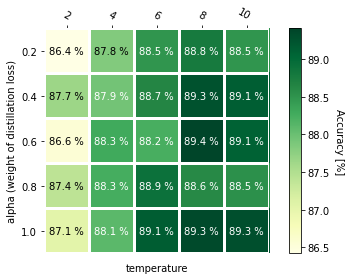
\includegraphics[width=0.7\linewidth]{fig/kd_2.png}
	\end{center}
	
	Some key observations from the above heatmap:
	\begin{itemize}
		\item Best improvement is of about \textbf{2.1\%}.
		
		\item The given student-teacher pair works best for high temperature due to high confidence of teacher model.
		
		\item When $\alpha = 1$, this means no use of labels but still we get \textbf{2\%} improvement.
	\end{itemize}
	
	
	\begin{table}[!htbp]
		\centering
		\caption{Comparison of models for CIFAR-10 Dataset}
		\label{tab:my-table}
		\begin{tabular}{@{}cll@{}}
			\toprule
			\textbf{Model} & \multicolumn{1}{c}{\textbf{Size}} & \multicolumn{1}{c}{\textbf{No. of Parameters}} \\ \midrule
			Teacher Model  & 86 MB                           & 11,183,562
			\\
			Student Model  & 9 MB                            & 816,938                                        \\ \bottomrule
		\end{tabular}
	\end{table}
	
	\subsection{Experiment 3: Variation with Amount of Training Data} 
	The motivation of this experiment was that the dark knowledge contains more information than hard label, so the student model should be able to learn from less data.
	\begin{itemize}
		\item \textbf{Dataset:} CIFAR-10 Dataset
		\item \textbf{Teacher Model:} ResNet 18
		\item \textbf{Student Model:} 6 Convolutional layers (with Batch Norm) + 2 FC layers.
	\end{itemize}
	We obtain the following results:
	
	\begin{center}
		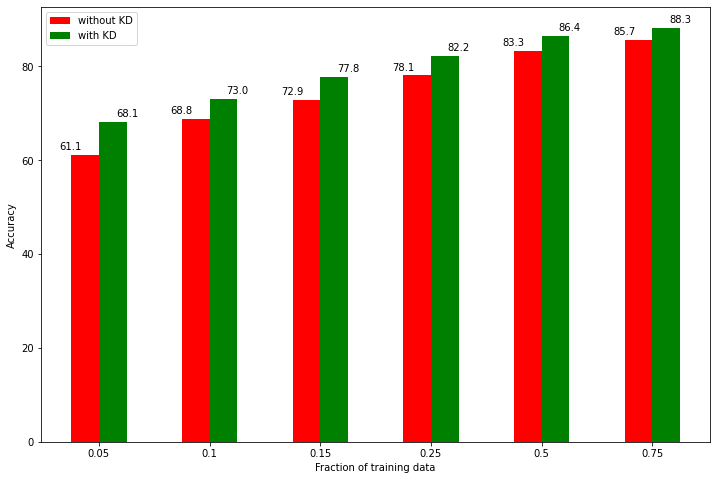
\includegraphics[width=0.9\linewidth]{fig/kd_3.png}
	\end{center}
	
	Some key observations from the above graph:
	\begin{itemize}
		\item Even with only \textbf{25\%} data, the accuracy achieved is comparable to the student model trained from scratch.
		
		\item The improvement due to Knowledge Distillation is more prominent for less data.
	\end{itemize}
	
	
	\subsection{Experiment 4: Teacher Free Knowledge Distillation}
	
	\begin{itemize}
		\item \textbf{Dataset:} CIFAR-10 Dataset
		\item \textbf{Student Model}: 6 Convolutional layers + 2 FC layers 
	\end{itemize}
	In this experiment we use the pre-trained student as a teacher (proposed by Yuan et al. \cite{teacherfree}) and find the accuracy for different values of $\alpha$ and $T$.
	
	\newpage
	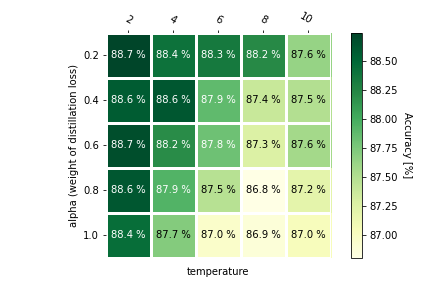
\includegraphics[scale=0.7]{fig/SSgrid.png}
	
	Using pre-trained student model as teacher has a regularizing effect and we achieve a maximum accuracy of \textbf{88.7\%} (+1.45\%). When we use high values of $T$, the distribution of teacher's soft predictions becomes similar to uniform distribution and has the same effect as Label Smoothing Regularization.\\
	The student model is smaller and predicts with lower confidence (softer probabilities) than a more complex model like ResNet-18, therefore it is able to obtain good accuracy at lower values of $T$.
	
	
	\subsection{Experiment 5: Distilled Student as Teacher}
	\begin{itemize}
		\item \textbf{Dataset:} CIFAR-10 Dataset
		\item \textbf{Student Model}: 6 Convolutional layers + 2 FC layers 
	\end{itemize}
	In this experiment we use the pre-trained \textbf{distilled} student model ($\alpha=0.6$ and $T=2$) from the previous experiment as teacher. We try different values of $\alpha$ and $T$ and observe that for $\alpha=0.4$ and $T=4$ the student model attains an accuracy of $\mathbf{89\%}$ which is close to the maximum accuracy ($\mathbf{89.4\%}$) obtained by using ResNet-18 as teacher. 
	Distilled student gives soft predictions with better confidence than a normal student when used as a teacher which explains the maximum accuracy obtained in this experiment is at $T=4$ instead of $T=2$.
	
	\subsection{Experiment 6: Using Teaching Assistants}
	\textbf{Problem:} Gap between student and teacher model affects the knowledge transfer. \\
	We conducted experiments with 5 different models which are differentiable in terms of number of convolutional layers: 2, 4, 6, 8, 10.\\
	Note that all models are regularized properly and trained for 100 epochs using SGD
	
	\textbf{Abbreviations used: } T: Teacher Model size, S: Student Model Size
	
	Below in figure \ref{Teacher_size} and \ref{Teacher_student_size} are the empirical results for evidence of the above problem:
	\begin{itemize}
		\item The left graph shows that even though the teacher model is improving in terms of accuracy (as shown in fig \ref{Teacher_size}), but still the student model (S = 2) is not able to benefit from that using knowledge distillation.
		
		\item Similarly, the right graph shows that the variation of gain in accuracy with different student sizes.
	\end{itemize}
	
	\newpage
	\begin{center}
		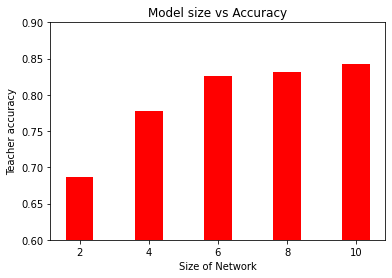
\includegraphics[width=0.6\linewidth]{fig/kd_13.png}
		\captionof{figure}{Model Size vs Accuracy}
		\label{Teacher_size}		
	\end{center}
	
	\begin{center}
		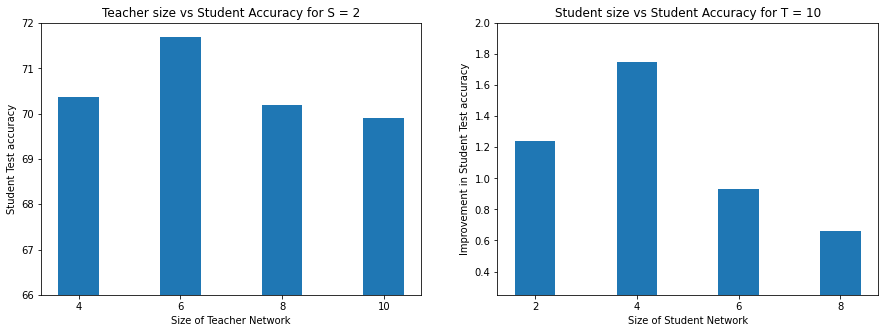
\includegraphics[width=\linewidth]{fig/kd_14.png}
		\captionof{figure}{a) Teacher size vs Student Accuracy  b) Student Size vs Gain in Student Accuracy}
		\label{Teacher_student_size}
	\end{center}
	
	These are the reasons that are mentioned in the paper\cite{assistant} and seemed very logical are as following:
	\begin{itemize}
		\item Teacher’s performance increases, thus it provides better supervision for the student by being a better predictor. 
		
		\item The teacher is becoming so complex that the student does not have the sufficient capacity or mechanics to mimic her behavior despite receiving hints. 
		
		\item Teacher’s certainty about data increases, thus making its logits (soft targets) less soft. This weakens the knowledge transfer which is done via matching the soft targets.
	\end{itemize}
	
	Reason number 1 is stating that the knowledge transfer is beneficial when the gap between student and teacher model is big, whereas other 2 reasons tells why that would not be so.
	
	\textbf{Using TA's to bridge the gap}: achieved the following results: \\
	\textbf{Student Size: } 2 conv layers, \textbf{Teacher Size: } 10 conv layers 
	
	\begin{table}[!htbp]
		\centering
		\caption{TA Size vs Student Accuracy}
		\label{tab:my-table}
		\begin{tabular}{@{}cllll@{}}
			\toprule
			\textbf{No KD} & \multicolumn{1}{c}{\textbf{Baseline KD}} & \multicolumn{1}{c}{\textbf{TA size = 4}} & \multicolumn{1}{c}{\textbf{TA size = 6}} & \multicolumn{1}{c}{\textbf{TA size = 8}}\\ \midrule
			68.6\%  & 71.1\%  &  71.5\%  &  72.5\%  &  72.1\%  \\ \bottomrule
		\end{tabular}
	\end{table}
	
	\section{Tools and Softwares used}
	All our models were implemented using Tensorflow \cite{abadi2016tensorflow} and Keras \cite{chollet2015keras}. Tensorflow is an automatic differentiation framework, which has become really popular for Deep Learning models. %Using the library, one can define the forward propagation in arbitrary computational graphs, and the library will compute the backpropagation itself. It also optimizes the graph for faster computation GPU, and provides various implementations of popular optimizers like RMSProp, Adam etc.%
	It allows us to customize the entire training and testing process which was very essential for this project.\\
	Keras is a high-level API that is built on top of TensorFlow. It is extremely user-friendly and comparatively easier than TensorFlow but offers less flexibility.\\
	We trained our models on Google colab notebooks using GPU as hardware accelerator. 
	All python notebooks and models can be obtained at \href{https://github.com/vaithak/Knowledge\_Distillation}{\color{blue}{https://github.com/vaithak/Knowledge\_Distillation}}
	
	
	\section{Learnings from the Project}
	\begin{itemize}
		\item One of the main learnings that we got from this project is realizing that deep learning is more than just implementing big neural networks and training them on a heavy machine. There are many insights and learning that one can get, if one thinks more about the inner workings and intricacies of machine learning.
		
		\item We also got more deep insights into the learning process of deep neural networks as we also had to read many papers and articles even before writing a single line of code.
		
		\item We became more familiar with implementing deep learning models, going from an idea to implementation quickly with the help of frameworks like Tensorflow. Also, for the project we had to implement custom learning rate scheduler, custom training step and custom loss function which gave us even more insight to the framework than just using the prebuilt functions.
		
	\end{itemize}
	
	\section{Future Work}
	Although in our complete project, we did analysis of cases when knowledge is transferred from the logits of teacher model. As stated in the literature review section, there have been a good amount of work in which along with the output logits, the teacher also provides hints to the student using output of the inner feature maps. This can be explored more in the future.
	
	All our empirical analysis was mainly for classification models, as mentioned in the literature review, there also has been some work on knowledge distillation for object detection models \cite{NIPS2017_e1e32e23} . This can be analysed empirically in future.
	
	\bibliography{references}
	
	%\section{References}
	% may use bixtex to automatically generate the list of references or
	% enter these manually below
	
	%\small{
	%[1] Reference 1
	
	%[2] Reference 2
	%}
	
\end{document}
